\documentclass[spanish, fleqn]{article}
\usepackage{babel}
\usepackage[utf8]{inputenc}
\usepackage{amsmath}
\usepackage{amsfonts}
\usepackage{mathrsfs}
\usepackage{dcolumn}
\usepackage[colorlinks, urlcolor=blue]{hyperref}
\usepackage{fourier}
\usepackage{tikz}
\usepackage{float}
\usetikzlibrary{arrows,shapes,snakes,automata,backgrounds,petri,babel,positioning}
\usepackage{pgf}
\usepackage[top = 2.5cm, bottom = 2cm, left = 2cm, right = 2cm]{geometry}
\definecolor{navyblue}{RGB}{0,148,222}
\definecolor{supercolor}{RGB}{0,148,12}
\tikzstyle{transition}=[rectangle,thick,draw=black!75,fill=black!20,minimum size=8mm]

\newcommand{\num}{1}

\title{INF-155: Introducción a la Informática Teórica\\
       [0.4\baselineskip]
       Tarea \#2 \\
       \emph{``Now it’s my fault''}
      }
\author{\href{mailto:roberto.fuentes@alumnos.usm.cl}{Roberto Fuentes}\\
201173037-2}
\date{4 de Mayo 2017}

\begin{document}
\maketitle

\thispagestyle{empty}

\section*{Solución}
    
    \begin{enumerate}

        \item 
        \begin{enumerate}
            \item Para esto, tomaremos los siguientes lenguajes:
            \begin{enumerate}
                \item $\mathcal{L}_1$ = Lenguaje \textbf{no regular} que contiene un simbolo $\alpha$. 
                \item $\mathcal{L}_2$ = Complemento de $\mathcal{L}_1$ unido con el simbolo $\alpha$, es decir, $\overline{\mathcal{L}_1} \cup \{\alpha\}$
            \end{enumerate}
            
            Teniendo esto, realizaremos la concatenación entre ellos:
            \begin{align*}
                \mathcal{L}_1 \mathcal{L}_2 = \mathcal{L}_1 \overline{\mathcal{L}_1} \cup \mathcal{L}_1 \cup \overline{\mathcal{L}_1} \cup \{\alpha\} = \Sigma^*
            \end{align*}
            
            lo cual nos quedó un lenguaje que es \textbf{regular}, por lo que si $\mathcal{L}_1$ $\cdot \mathcal{L}_2$ o $\mathcal{L}_2$ $\cdot \mathcal{L}_1$ no asegura que $\mathcal{L}_1$ sea regular.
            \item Teniendo en cuenta que $\mathcal{L}_1$ y 	$\mathcal{L}_2$ son regulares, la diferencia $\mathcal{L}_1$ - 	$\mathcal{L}_2$ puede ser expresada por teoria de conjuntos de la siguiente forma:
            
            \begin{align*}
                \mathcal{D} \mathfrak{i f f} = \mathcal{L}_1 - \mathcal{L}_2 = \mathcal{L}_1 \cap \overline{\mathcal{L}_2} 
            \end{align*}
            
            Es decir, puede ser expresado como el conjunto de cadenas que pertenecen a $\mathcal{L}_1$ y no pertenecen a $\mathcal{L}_2$, lo que se traduce a la intereseccion de $\mathcal{L}_1$ con el complemento de $\mathcal{L}_2$, operaciones que son cerradas y ademas al aplicarlas en nuestros lenguajes, siguen siendo regulares. Por lo tanto, concluimos que $\mathcal{L}_1 - \mathcal{L}_2$ es regular.
            
            \item Analizando cada una de las condiciones que nos dan, por propiedades de clausura nos damos cuenta de que cada condición es regular, ya que cumple con operaciones bajo las cuales los lenguajes regulares son cerrados, por lo que el lenguaje es regular.
        \end{enumerate}
        
        \item Nos piden demostrar si $L = \{x^i y^j z^k \mid i \leq 2j \text{ ó } j \leq 3k \}$ es regular o no usando lema del bombeo. Para esto, primero asumiremos que este lenguaje es regular. Luego, demostraremos por contradicción lo contrario, y aplicaremos lema del bombeo. 
        Sea $N \geq 1$ la constante del lema del bombeo, elegimos $\sigma = x^N y^\frac{N}{2} z^0$, donde $\mid \sigma \mid = N+\frac{N}{2} > N$. Es importante destacar que cumple con la primera condicion ($i\leq 2j$), pero no cumple con la segunda ($j\leq3k$). Siendo asi, por \textbf{lema del bombeo} podemos escribir $\sigma$ como una cadena $\alpha\beta\gamma$, donde la cantidad de elementos de $\alpha\beta$ no puede superar a N ($\mid\alpha\beta\mid\leq N$), además $\beta\neq\epsilon$, y para todo $k\geq 0$ se debe cumplir que $\alpha\beta^k \gamma$ debe pertenecer a $L$. Siendo así, tenemos lo siguiente:
        
        \begin{align*}
           \underbrace{xx\ldots x}_{N}\mid \underbrace{yy\ldots y}_{\frac{N}{2}}
        \end{align*}
        
        Por lo que la cadena $\alpha\beta$ serian a lo mas todas las $x$ posibles, por lo que podemos dejar la cadena de la siguiente forma:
        
         \begin{align*}
            \underbrace{xx\ldots x}_{\alpha}\mid \underbrace{yy\ldots y}_{\beta} \mid
            \underbrace{yy\ldots y}_{\gamma}
        \end{align*}
        
       Nos damos cuenta que al bombear $k$ (hacer crecer $k$), la cadena de $x$ aumenta, mientras que las $y$'s quedan del mismo largo. Si hacemos k = 1, nos queda que:
       \begin{align*}
            N+1 \leq 2\cdot \frac{N}{2} \\
            N+1 \leq N
       \end{align*}
       
       Rompiendo la condición de $i \leq 2j$,y en conjunto con no cumplir $j \leq 3k$ llegamos a una \textbf{contradicción}, concluyendo que el lenguaje $L$ \textbf{no es regular}.
       
       
        \item Primero debemos considerar que la lista en $scheme$ debe comenzar con un $" ' ( "$, añadiendo el elemento $A$ al $stack$. Posteriormente, puede venir un \textcolor{red}{parentesis abierto} o un \textcolor{blue}{elememto teminal $\alpha$}. Para el primer caso añadimos $A$ a la pila, y para el segundo caso añadimos $B$. Posteriormente, podemos seguir abriendo parentesis, o seguir añadiento elementos terminales segun sea el caso. Cabe señalar que si se añade un simbolo terminal, también se añade un símbolo $"$  $"$ a los terminales, y el elemento $C$ a la pila. Luego, al sacar los elementos $A$ del $stack$, debemos añadir $)$ a la lista, y al sacar $B$ o $C$, agregaremos $\epsilon$. Podemos seguir agregando parentesis o simbolos terminales, pero al quedar vaciada la pila, la cantidad de parentesis abiertos y cerrados \textbf{seran siempre iguales}, por lo que creariamos una lista con posibilidad de tener listas anidadas con elementos dentro. El PDA que refleja lo explicado se presenta a continuación:
        
        \begin{center}
        	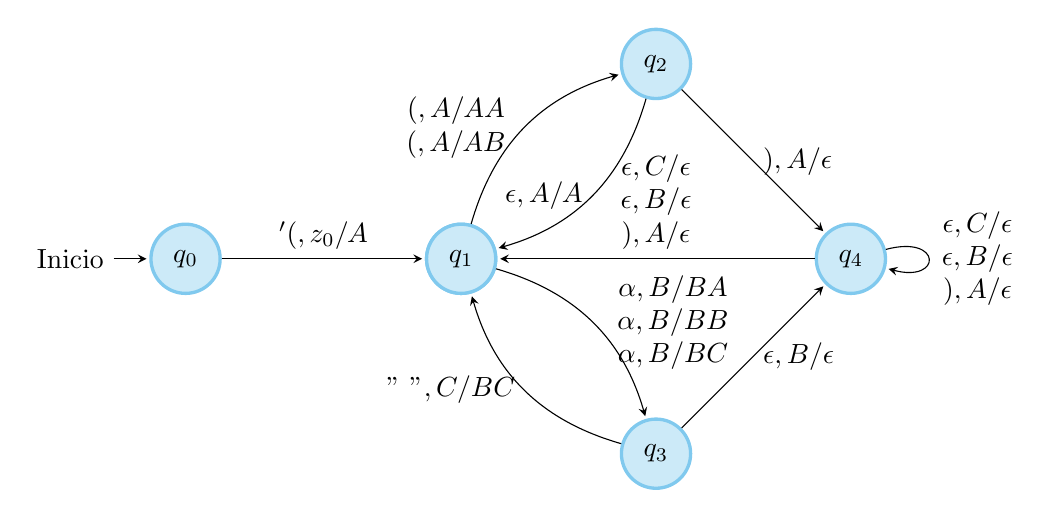
\begin{tikzpicture}[shorten >=1pt,node distance=3.5cm,on grid, >=stealth, initial text=Inicio, every state/.style={draw=navyblue!50,very thick,fill=navyblue!20}, bend angle=35]]
        		\node[state,initial]    (q_0)                        {$q_0$};
                \node[state]	        (q_1) [right of = q_0]       {$q_1$};
                \node[state]	        (q_2) [above right of = q_1] {$q_2$};
                \node[state]	        (q_3) [below right of = q_1] {$q_3$};
                \node[state]	        (q_4) [below right of = q_2] {$q_4$};
                \node[state]	        (q_1) [right of = q_0]       {$q_1$};
            \path[->]   (q_0) edge node [above]                 {$'(,z_0 / A$} (q_1)
                        (q_1) edge[bend left=29] node[left,text width=1.5cm,align=center]    {$(,A/AA$\\$(,A/AB$} (q_2)
                        (q_2) edge[bend left=29] node [left]   {$\epsilon,A/A$} (q_1)
                        (q_1) edge[bend left=29] node  [right,text width=1.8cm,align=center] {$\alpha,B/BA$\\$\alpha,B/BB$\\$\alpha,B/BC$} (q_3)
                        (q_3) edge[bend left=29] node [left]    {$"\ ",C/BC$} (q_1)
                        (q_2) edge node [right]                 {$),A/ \epsilon$} (q_4)
                        (q_3) edge node [right]                 {$\epsilon, B/ \epsilon$} (q_4)
                        (q_4) edge node [above,text width=1cm,align=center] {$\epsilon,C/ \epsilon$\\$\epsilon,B/ \epsilon$\\$),A/\epsilon$} (q_1)
                        (q_4) edge[loop right] node[text width=1cm,align=center] {$\epsilon,C/ \epsilon$\\$\epsilon,B/ \epsilon$\\$),A/\epsilon$} (q_4);
        	\end{tikzpicture}
    	\end{center}
    	
    	\item Nos piden justificar si es posible llevar el lenguaje $\mathcal{L} = \{b^{2r} a^{n+1} d^j e^{r+1} /n,r \geq 0 \wedge j > r \}$ con $n,r,j \in$ $\mathbb{N}_0$ a la forma normal de Chomsky. Para esto, debemos ver primero si el lenguaje es de $contexto$ $libre$, por que usaremos contradicción junto a el \textbf{lema del bombeo para lenguaje de contexto libre} para demostrar que este lenguaje no es de contexto libre. Sea $\mathcal{L}$ un $CFL$, hacemos $\sigma = B^0 A^{N+1} D^{1} R^{0+1} \in L$, donde $\mid\sigma\mid = N+3 >N$. Por PLCFL, existe un $u,v,w,x,y \in \Sigma^*$ tales $\mid vwx \mid \leq N, vx \neq \epsilon$ tales que para todo $k\leq0$ se tiene que $uv^kwx^ky \in L$. Al tomar esto, tenemos varios casos que puede tomar la cadena $\mid vwx \mid$. Tomaremos el caso de $\mid vwx \mid = E$. Haciendo esto, al bombear $k$, aumentará el número de $E$, haciendo se rompa la condición $j>r$, y por \textbf{contradicción} nuestro lenguaje $L$ no cumple con el PLCFL, y finalmente no se podría llevar a la forma normal de Chomsky.
 
    \end{enumerate}

    
\end{document}